% http://kleinmann.eit.h-da.de/99_ThesisInfos/

\section{Einführung / Problembeschreibung} 
\subsection{Was ist die Motivation?}
\subsection{Was ist die Aufgabe?}
\subsection{Was ist das Ziel dieser Arbeit?}
\subsection{Was war der Status Quo, bevor mit dieser Arbeit begonnen wurde?}
\subsubsection{Firma X hat etwas in Vergangenheit auf diesem oder jenem Wege gemacht…}
\section{Problemlösung}
\subsection{Was sind die Optionen / Welche prinzipiellen Lösungen sind möglich?}
\subsection{Stand der Technik / Wie wird es woanders gemacht?}
\subsection{Was ist der in dieser Arbeit gewählte Ansatz?}
\subsection{Weshalb wurde dieser Ansatz gewählt / Was unterscheidet ihn von anderen / Was ist neu / Was ist bekannt?}
\subsection{Detaillierte Beschreibung der Problemlösung}
\section{Implementierung und Test}
\subsection{Wie wurde es implementiert}
\subsection{Wie wurde getestet}
\subsection{why was it tested the way it was tested?}
\section{Validierung}
\subsection{Was sind die Ergebnisse}
\subsection{Vor- und Nachteile des entwickelten Systems}
\section{Zusammenfassung / Fazit / zukünftige Arbeit}
\subsection{Was wurde getan}
\subsection{Was muss noch getan werden / Wie kann das System verbessert werden?}


%\section{Einführung}
%Jemand "`musste"' Josef K. verleumdet haben, denn ohne dass er etwas Böses getan hätte, wurde er eines Morgens verhaftet. »Wie ein Hund!« sagte er, es war, als sollte die Scham ihn überleben. Als Gregor Sams eines Morgens aus unruhigen Träumen erwachte, fand er sich in seinem Bett zu einem ungeheuren Ungeziefer \index{Ungeziefer} verwandelt. Und es war ihnen wie eine Bestätigung ihrer neuen Träume und guten Absichten, als am Ziele ihrer Fahrt die Tochter als erste sich erhob und ihren jungen Körper dehnte \cite[S.55ff]{Accardi.2010}. »Es ist ein eigentümlicher Apparat«, sagte der Offizier zu dem Forschungsreisenden und überblickte mit einem gewissermaßen bewundernden Blick den ihm doch wohlbekannten Apparat \ac{KDE}. Sie hätten noch ins Boot springen können, aber der Reisende hob ein schweres, geknotetes Tau vom Boden, drohte ihnen damit und hielt sie dadurch von dem Sprung ab. In den letzten Jahrzehnten ist das Interesse an Hungerkünstlern sehr zurückgegangen. Aber sie überwanden sich, um drängten den Käfig und wollten sich gar nicht fort rühren. Jemand musste Josef K. verleumdet haben, denn ohne dass er etwas Böses getan hätte, wurde er eines Morgens verhaftet. »Wie ein Hund!« sagte er, es war, als sollte die Scham ihn überleben \cite{Lewis.2010}.
%
%\begin{figure}[h]
%\centering 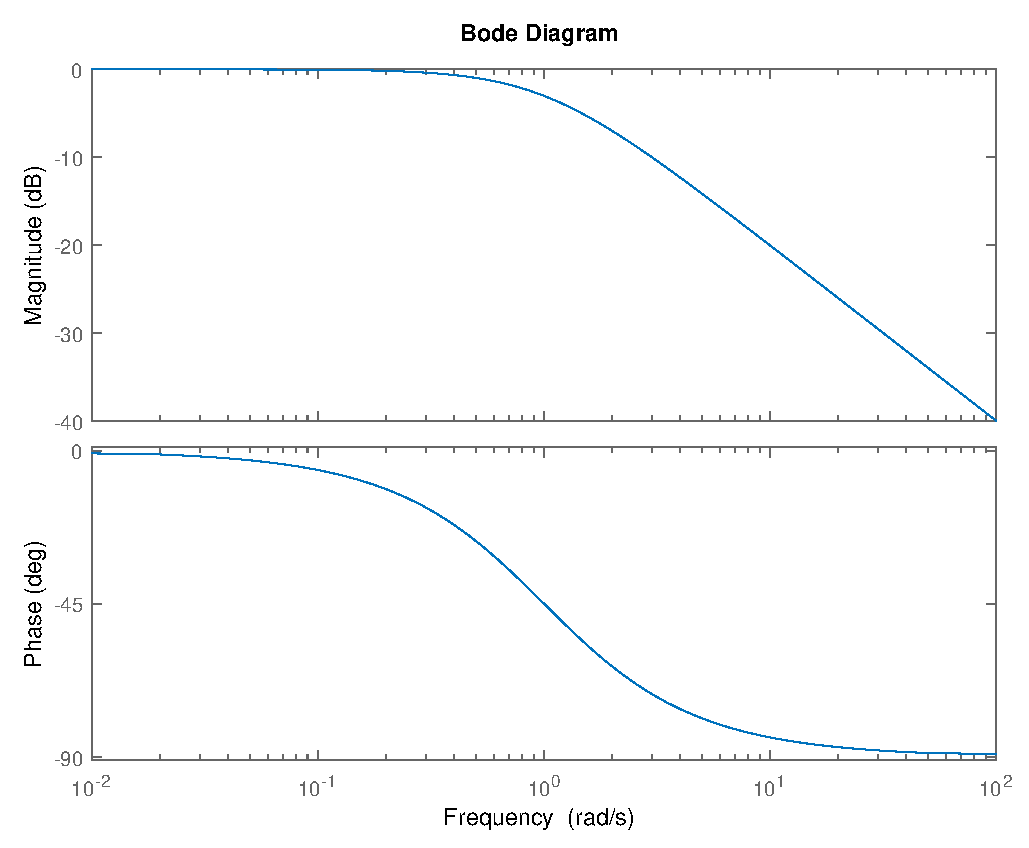
\includegraphics[width=0.5\textwidth]{fig/PT1/PT1.eps}
%\caption{Bodediagramm PT1}
%\end{figure}
%
%\subsection{Motivation}
%Als Gregor Sams eines Morgens aus unruhigen Träumen erwachte, fand er sich in seinem Bett zu einem ungeheuren Ungeziefer verwandelt. Und es war ihnen wie eine Bestätigung ihrer neuen Träume und guten Absichten, als am Ziele ihrer Fahrt die Tochter als erste sich erhob und ihren jungen Körper dehnte. »Es ist ein eigentümlicher Apparat«, sagte der Offizier zu dem Forschungsreisenden und überblickte mit einem gewissermaßen bewundernden Blick den ihm doch wohlbekannten Apparat.
%
%\begin{IEEEeqnarray}{rCl}
%	a & = & b + c \\
%	& = & d + e + f + g + h \\
%	& = & p + q + r + s
%\end{IEEEeqnarray}
%
% Sie hätten noch ins Boot springen können, aber der Reisende hob ein schweres, geknotetes Tau vom Boden, drohte ihnen damit und hielt sie dadurch von dem Sprung ab. In den letzten Jahrzehnten ist das Interesse an Hungerkünstlern sehr zurückgegangen. Aber sie überwanden sich, um drängten den Käfig und wollten sich gar nicht fort rühren.Jemand musste Josef K. verleumdet haben, denn ohne dass er etwas Böses getan hätte, wurde er eines Morgens verhaftet.
%
%\begin{table}[h]
%	\centering
%	\begin{tabular}[h]{|c|c|}
%		\hline
%		$U_e$ / V& $U_a$ / V\\ \hline
%		0.1 & 0.2 \\ \hline
%		0.2 & 0.4 \\ \hline
%		0.3 & 0.6 \\ \hline
%		0.4 & 0.8 \\ \hline
%		0.5 & 1 \\ \hline
%	\end{tabular}
%	\caption{Messergebnisse}
%\end{table}
%
%»Wie ein Hund!« sagte er, es war, als sollte die Scham ihn überleben. Als Gregor Sams eines Morgens aus unruhigen Träumen erwachte, fand er sich in seinem Bett zu einem ungeheuren Ungeziefer verwandelt \cite{Pleisteiner.2007}.
